\chapter{Anhang}

\section{Projektanforderungen}
\label{projektanforderungen}
Das Projekt wird im Rahmen des IP5 an der FHNW durchgeführt. Sein Hauptziel ist es, ein Plugin für das Datenanalyse-Tool Gephi zu entwickeln, mithilfe wessen Vorhersagen möglicher neuer Kanten zwischen Knoten in einem Netzwerk durchgeführt werden können. Solche Vorhersagen neuer Verbindungen zwischen zwei Knoten werden Link Predictions genannt. Das Projekt wird von Michael Henninger betreut und wurde auch von ihm in Auftrag gegeben.
Die genauen Vorgaben für die Umsetzung lauten, wie folgt:

\begin{itemize}
    \item Von den verschiedenen, existierenden Link Prediction Algorithmen soll mehr als einer ausgewählt und in das Plugin eingebaut werden.
    \item Da das Plugin am Schluss als Open Source Projekt zur Verfügung gestellt werden soll, muss es umfassend dokumentiert, gut getestet und bezüglich der Algorithmen leicht erweiterbar gestaltet werden.
    \item Es muss eine geeignete Visualisierung und Datenstruktur gefunden werden, um die vorausgesagten Kanten in einem Netzwerk darzustellen. Dazu müssen mindestens simple Entwürfe skizziert und abgenommen werden.
    \item Darüber hinaus soll es die Möglichkeit geben, zwei Netzwerke zu verschiedenen Zeitpunkten zu vergleichen und zu berechnen, mit welchem der implementierten Link Prediction Algorithmen die beste Vorhersage gemacht worden wäre. Auch hierfür ist es essentiell, eine geeignete Visualisierung und Datenstruktur zu bestimmen.
    \item Die vorhergesagten Kanten sollen speziell markiert werden. So können diese beispielsweise eine neue Spalte mit Schwellwerten/Wahrscheinlichkeiten erhalten. Kanten, die es dabei schon von Anfang an gegeben hat, bekommen dabei einen Default-Wert wie 0 oder NULL.
\end{itemize}

\newpage

\section{Proof of Concept}
\label{poc}

Für die Einarbeitung in die Gephi-Plugin Entwicklung und erste Ansätze für die Umsetzung des Projekts zu finden, hat
sich das Projektteam entschlossen, ein Proof of Concept durchzuführen.

\subsection{Ziel}

Mit dem Proof of Concept, soll sich einerseits mit dem \ac{api} von \acs{gephi} vertraut zu machen.
Andererseits soll die Funktionsweise von ersten Ideen und Konzepten überprüft werden.

\subsection{Umsetzungsprozess}

\begin{itemize}
    \item \textbf{Filter:} Filter werden in \acs{gephi} verwendet, um ein Netzwerk auf Knoten oder Kanten zu reduzieren, welche bestimmte Eigenschaften besitzen.
    In Bezug auf Link-Prediction wurde deshalb eine neue Filterkategorie eingeführt, unter welcher nach verschiedenen Prediction-Algorithmen gefiltert werden kann.
    Durch Auswahl eines Algorithmus können jene Kanten herausgefiltert werden, welche durch Anwenden des Algorithmus neu hinzugefügt werden.
    Der Filter wird dabei um ein \acs{ui}-Element ergänzt, bei welchem die Anzahl der hinzugefügten Kanten eingegrenzt werden kann.

    \item \textbf{Statistiken:} Die Wahrscheinlinkteit, dass sich eine neue Kante zwischen zwei Knoten bildet, entspricht einem berechneten Wert.
    Diese Berechnung wird mittels Statistiken angestossen. Die gesamte Logik und Berechnung der verschiedenen Algorithmen wird anschliessend
    durch verschiedene Statistik-Objekte gekapselt.

    Die Funktionsweise für das Implementieren von neuen Statistik-Objekten ist im Gephi-Plugin Bootcamp gut dokumentiert. Darauf aufbauend
    konnte ein neues Statistik-Objekt mit entstprechendem Button im \acs{ui} implementiert werden. Bei der Berechnung wurde der Algorithmsu
    ``Common Neighbours'' eingesetzt, bei welchem die Anzahl Nachbarn jedes Knotens gezählt werden.

    Für die Implementierung des Algorithmus konnten bestehende Funktionen von \acs{gephi} verwendet werden um die Knoten aus dem Graphen, respektive
    dessen Nachbarn auszulesen. Die berechneten Werte konnten anschliessend bereits im \acs{datalaboratory} abgelegt werden.

    % TODO: Redundant?
    %Da für die Umsetzung der Link Prediction aber nicht nur die direkte Anzahl der Nachbarn relevant ist, sondern vor allem
    %die Zahl der gemeinsamen Nachbarn zweier Knoten wurde auch dafür noch eine Statistik umgesetzt. Hier werden nacheinander
    %die Knoten durchgegangen und getestet, wie viele ihrer Nachbarn mit den Nachbarn eines anderen Knotens übereinstimmen.
    %Wenn es noch keine Kante zwischen den beiden Knoten gibt, wird eine neue hinzugefügt und die Anzahl der gemeinsamen
    %Knoten als neues Attribut eingefügt. Wenn es die Kante bereits gibt, wird nur das neue Attribut befüllt. Zusätzlich
    %gibt es ein Attriut, das anzeigt, ob die Kante hinzugefügt wurde oder ob sie schon existiert hat. Zur Berechnung der
    %gemeinsamen Nachbarn werden darüber hinaus nur Kanten gewertet, die nicht erst bei der Berechnung hinzugefügt worden
    %sind.

    Damit dem Graphen Kanten hinzugefügt werden können, während diese noch gelesen und überarbeitet werden, muss ein Write-Lock
    verwendet werden. Die Logik, welche für den Algorithmus ``Common Neighbours'' implementiert wurde, kann für die spätere Umsetzung
    grösstenteils wiederverwendet werden.
\end{itemize}

\subsection{Erkenntnisse}

Es konnten verschiedene Erkenntnisse aus der Umsetzung des Proof Of Concept gewonnen werden.
Zum einen war es sehr hilfreich, sich zum ersten Mal aktiv mit dem \acs{api} von \acs{gephi} zu beschäftigen. Besonders wichtig war
dabei die Erkenntnis, dass die Beispiele aus dem Bootcamp teilweise veraltet sind. Um solche Beispiele mit einer neuen \acs{gepi}-Version
und den dadurch unterschiedlichen \acs{API}s zum Laufen zu bringen, muss zusätzlich Aufwand eingerechnet werden.

Weiter konnte mithilfe des Proof Of Concepts sichergestellt werden, dass sämtliche Installationen, Konfigurationen und die
Entwicklungsumgebung korrekt funktionieren. Viele konfigurative Probleme konnten hier bereits erkannt und frühzeitig behoben werden.

Vom technischen Aspekt her konnten wichtige Erkenntnisse für die spätere Umsetzung gewonnen werden - beispielsweise
wie ein Gephi-Plugin aufgebaut ist. Diese Erkenntnisse fliessen direkt in die Überlegungen beim Entwurf der Software-Architektur ein.
% TODO: Redundant?
%Um ein Beispiel zu nennen, konnte nach der Umsetzung des
%Proof of Concept aber bereits festgelegt werden, wie sichergestellt werden kann, dass die Anzahl Algorithmen für die
%Link Prediction beliebig erweitert werden kann, nämlich indem diverse Informationen in separate Klassen ausgelagert
%werden und es für jeden Algorithmus eine eigene Subklasse gibt, die grundsätzlich nur noch die Umsetzung des Algorithmus
%implementiert, jedoch nichts mit dessen Aufruf zu tun hat.
\newpage

\section{README.md}
\label{readme}

% Split readme in 3 parts
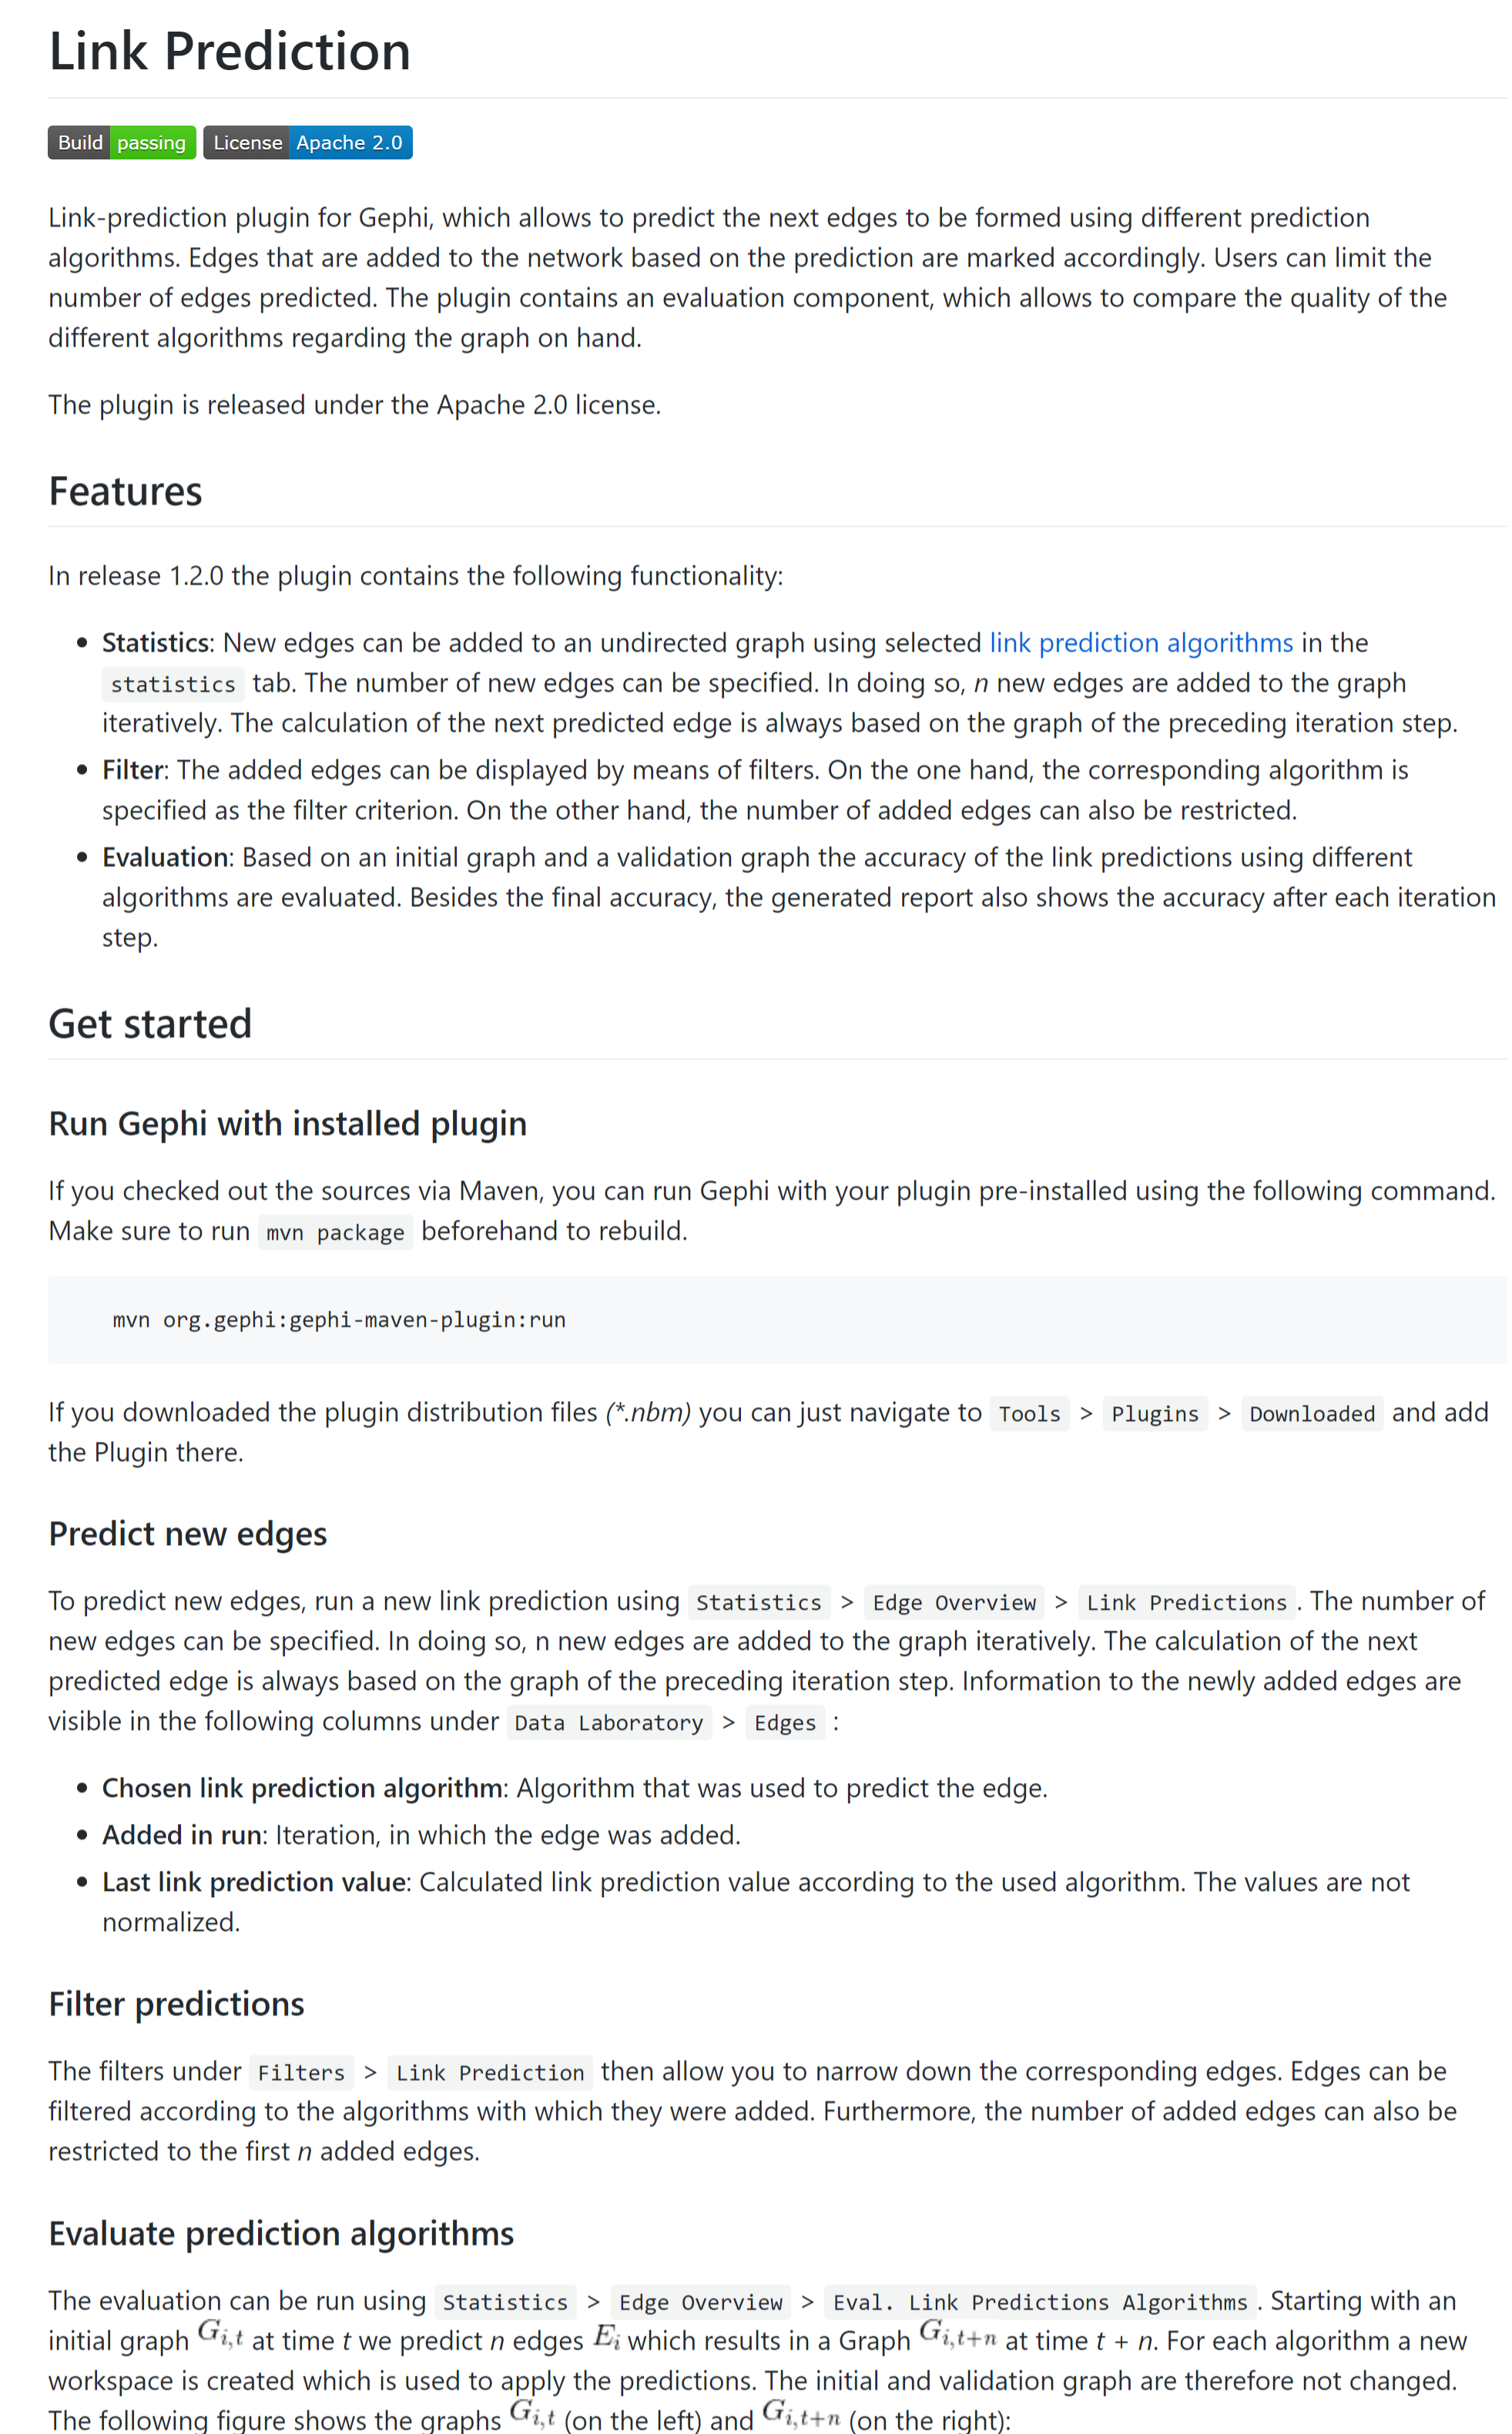
\includegraphics[width=\textwidth]{resources/readme_pt1.png}
\newpage
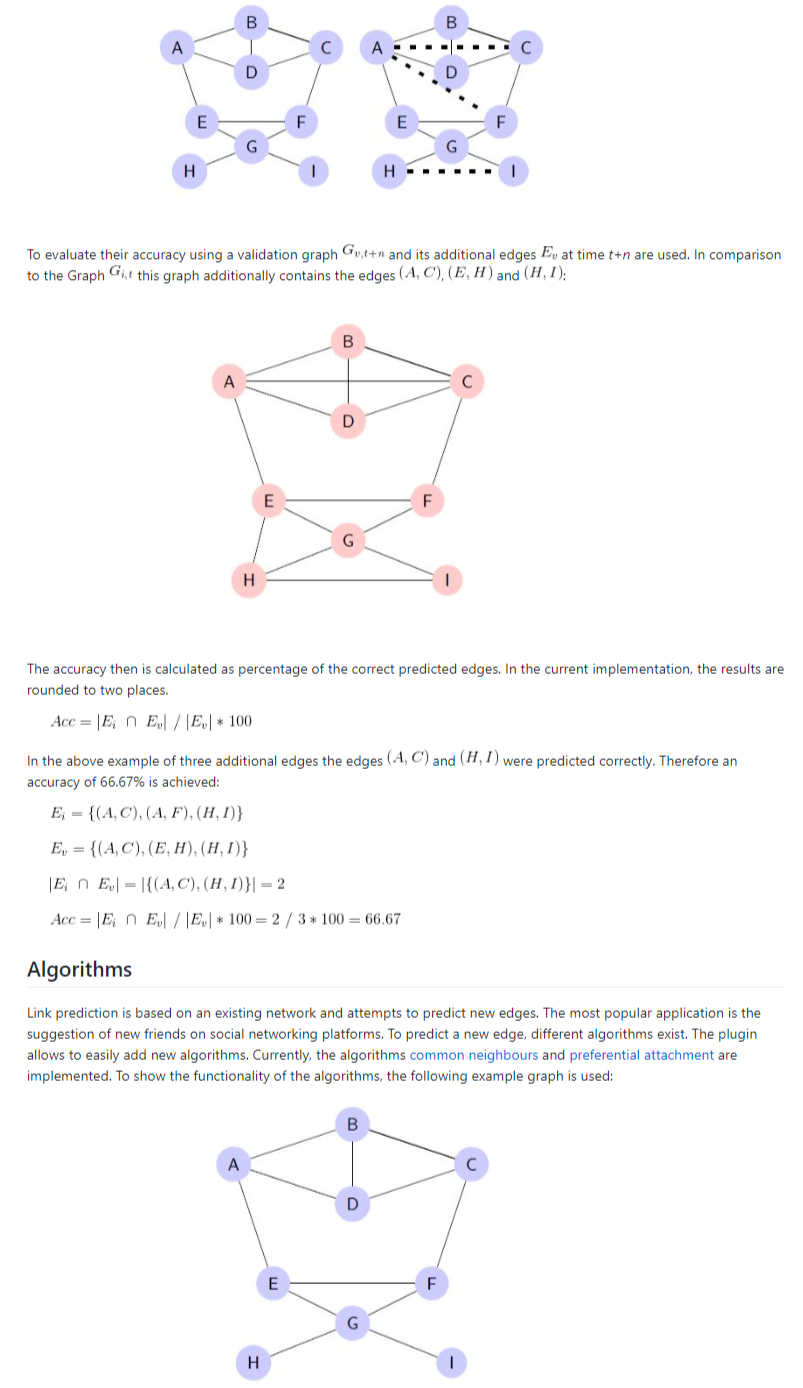
\includegraphics[width=\textwidth]{resources/readme_pt2.png}
\newpage
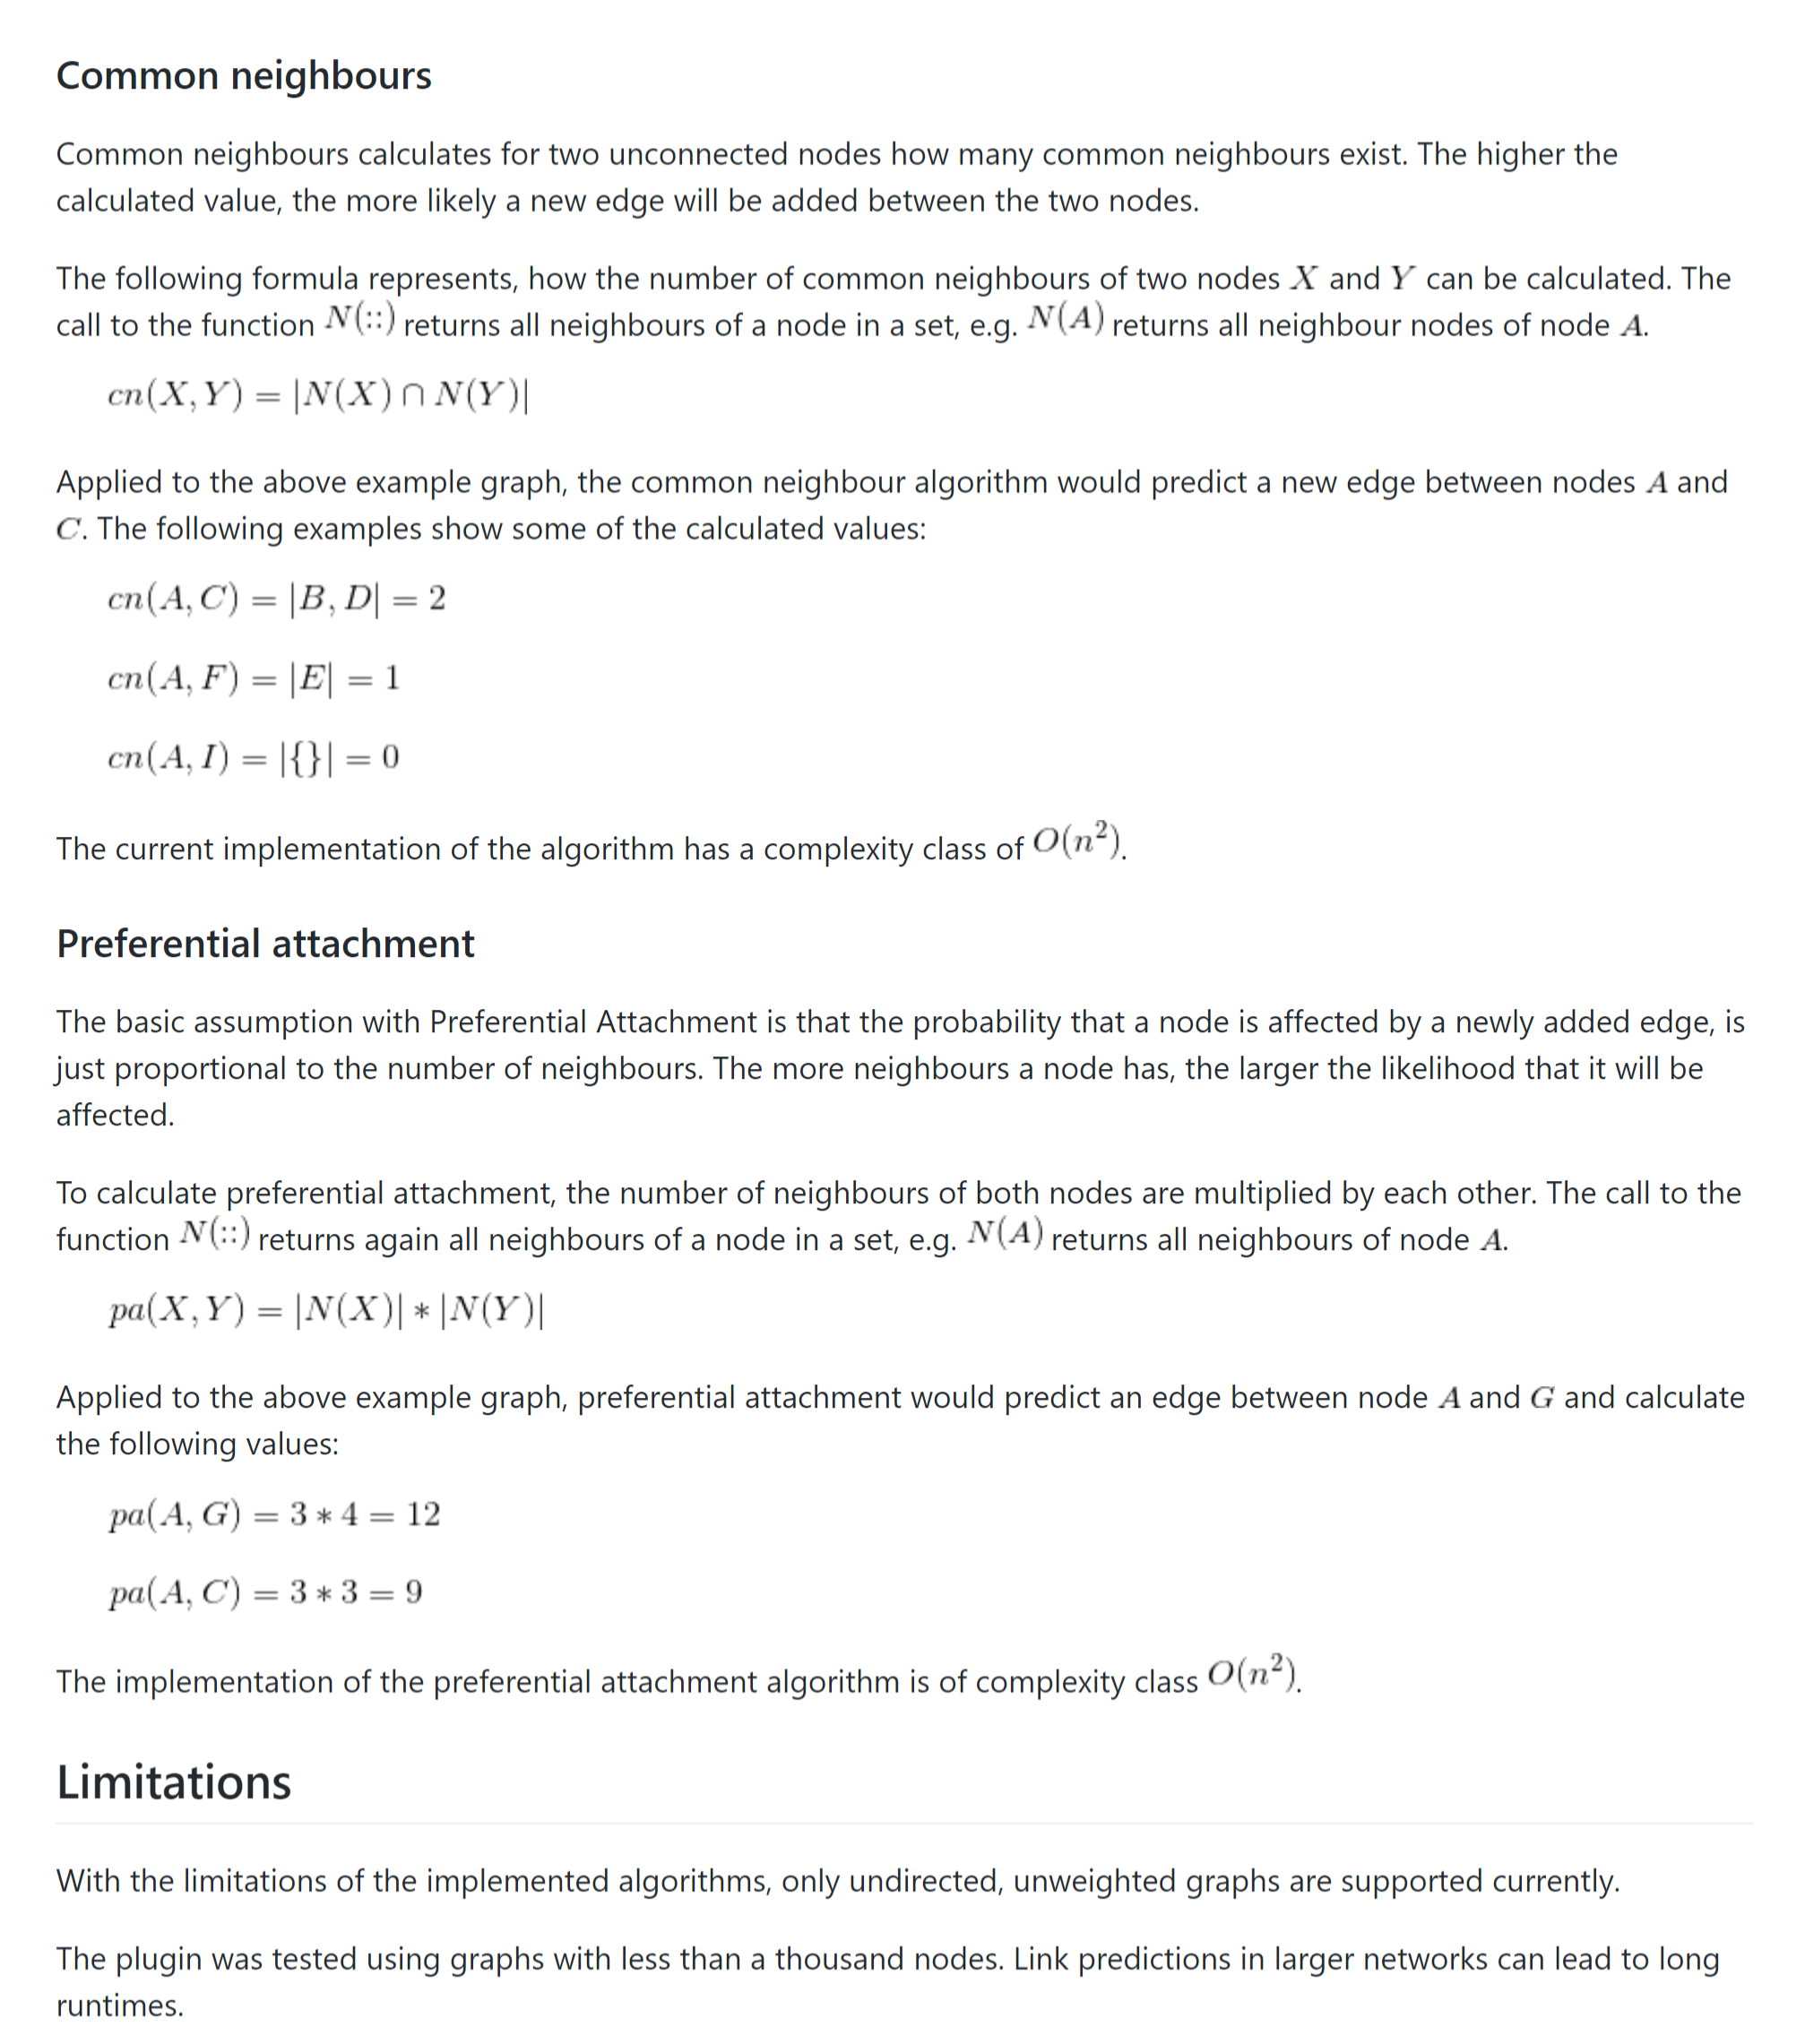
\includegraphics[width=\textwidth]{resources/readme_pt3.png}

%TODO: Add Exception/Error to Glossar


